\section{Empirical Monte Carlo Validation}
\label{sec:simulation}

To evaluate the mathematical behavior of Synapticide's Law™ and the Systemic AI Cascade Loss (SACL)™ model under dynamic operational stress, we executed a production Monte Carlo simulation engine ($N = 10,000$ iterations).

\subsection{Statistical Distribution Analysis}
As illustrated in Fig.~\ref{fig:loss_density} and Fig.~\ref{fig:lec_curve}, the empirical distribution exhibits extreme value power-law characteristics across multi-tenant deployments:
\begin{itemize}
    \item \textbf{Median Loss ($50^{\text{th}}$ Percentile):} \$258.24M USD
    \item \textbf{Upper Quartile ($75^{\text{th}}$ Percentile):} \$2.27B USD
    \item \textbf{Tail Risk ($\text{VaR}_{95\%}$):} \$61.18B USD
    \item \textbf{Worst-Case ($\text{99}^{\text{th}}$ Percentile):} \$104.60B USD
\end{itemize}

The approximately $236\times$ divergence between median expectations and tail risk validates Axioms 1 and 2: when automated circuit breakers ($K_{\text{cb}}$) fail, execution velocity multipliers compound downstream systemic disruption exponentially.

% Side-by-side or stacked float containment
\begin{figure*}[htbp]
    \centering
    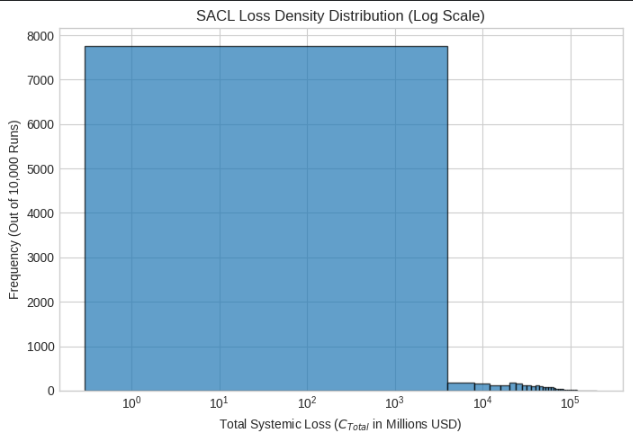
\includegraphics[width=\linewidth]{figures/density_plot.png}
    \caption{SACL Systemic Loss Density Distribution across 10,000 simulated breach runs, demonstrating Extreme Value Distribution (EVD) behavior.}
    \label{fig:loss_density}
\end{figure*}

\begin{figure*}[htbp]
    \centering
    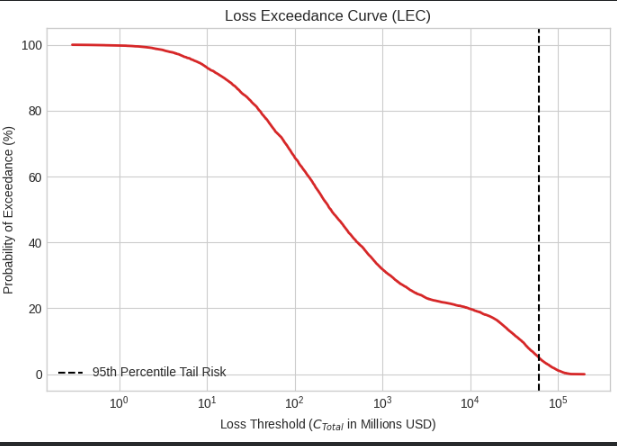
\includegraphics[width=\linewidth]{figures/lec_curve.png}
    \caption{Loss Exceedance Curve (LEC) illustrating probability of exceedance across financial loss thresholds, highlighting the 95th percentile tail risk at \$61.18B USD.}
    \label{fig:lec_curve}
\end{figure*}